\documentclass[11pt,a4paper]{article}
\usepackage[utf8]{inputenc}
\usepackage{amsmath}
\usepackage{mathtools}
\usepackage{amsfonts}
\usepackage{amssymb}
\usepackage{graphicx}
\usepackage{caption}
\usepackage{subcaption}
\usepackage{comment}
\usepackage{color}
\usepackage{enumitem}
\usepackage[left=2cm,right=2cm,top=2cm,bottom=2cm]{geometry}
\usepackage{listings}
\usepackage{color}

\setlength{\jot}{10pt}
 
\definecolor{codegreen}{rgb}{0,0.6,0}
\definecolor{codegray}{rgb}{0.5,0.5,0.5}
\definecolor{codepurple}{rgb}{0.58,0,0.82}
\definecolor{backcolour}{rgb}{0.95,0.95,0.92}
 
\lstdefinestyle{mystyle}{
    backgroundcolor=\color{backcolour},   
    commentstyle=\color{codegreen},
    keywordstyle=\color{magenta},
    numberstyle=\tiny\color{codegray},
    stringstyle=\color{codepurple},
    basicstyle=\footnotesize,
    breakatwhitespace=false,         
    breaklines=true,                 
    captionpos=b,                    
    keepspaces=true,                 
    numbers=left,                    
    numbersep=5pt,                  
    showspaces=false,                
    showstringspaces=false,
    showtabs=false,                  
    tabsize=2
}
 
\lstset{style=mystyle}
\graphicspath{ {./figures/} }
\author{Andrew Teta}
\title{ECEN 4532 - Lab 5: JPEG Image Processing}
\date{April 15, 2019}

\begin{document}

\maketitle

\begin{figure}[ht]
	\centering
	
\includegraphics[width=0.5\textwidth]{aic-logo}
\end{figure}

\pagebreak

\tableofcontents

\pagebreak

\addcontentsline{toc}{section}{Introduction}
\section{Introduction}
JPEG (Joint Photographic Experts Group) is a common compression scheme and file type used for image data compression and storage. JPEG is very common as it is efficient and easily implemented. This lab is an exercise in implementing the framework of the JPEG algorithm.

\section{Background}
\subsection{Why Compress Images?}
Image data is collected from many different sources in many different resolutions. Some examples would be camera pictures, medical (X-Ray, MRI, etc.), and video. Some of these are originally captured in analog format on tape or film media and some are inherently digital, such as a digital camera or video recorder. There are many reasons why a digital media format may be advantageous. For example:

\begin{itemize}
\item Storage and transmission 
\item Further processing (color correction, enhancement, crop, machine vision, etc)
\item Database storage
\end{itemize}

Storing images and videos in digital form at full resolution, especially for analog formats, introduces large hurdles for storage capacity and efficiency. Full resolution can also be called uncompressed and uncompressed data can make it more difficult to store, transmit, and search the data. Thus, there is motivation for some way to encode a lot of data in a small number of bits, neglect unnecessary information, or combine these both into a single 'compression scheme'.

\subsection{Compression}
At a high level, compression can be decomposed into the three components of (1) an encoder, (2) a decoder, and (3) a channel. A channel can be considered the media transmission platform. Examples include: wireless, satellite, ethernet, CD, optical fiber, computer memory, etc.

There is potential for transmission errors to occur in the channel, such as bit corruption over a wireless communication or something similar, however we will consider for this lab, only a perfect channel.

\subsection{Encoder}
JPEG is a transform-based encoder so we will focus on that, although there are others. A transform encoder can be decomposed into

\begin{enumerate}
\item Pre-processing. These would be things that occur before the actual compression algorithm with the purpose of preparing the data to minimize coding complexity or increase compression efficiency. Some examples would include:
	\begin{itemize}
	\item filtering
	\item zero-padding
	\item symmetric extension on the boundaries
	\item tiling
	\end{itemize}
\item Transform. The transform is intended to reduce the correlation among image pixels and describe most of the information in an image with a small set of significant coefficients. Then, most of the energy is condensed into a few coefficients.
\item Quantization. The transform output is a set of real-valued coefficients. The purpose of quantization is to represent these values with a much smaller set of values, often more easily represented within the encoding scheme. Quantization is non-reversible and distortion inducing. Image quality is balanced against the number of bits necessary to represent the data here.
\item Entropy coding. This is a creatively efficient way to reduce bit quantity. More common symbols (or information) is represented with shorter code-words and vice-versa.
\end{enumerate}

\subsection{Decoder}
The decoder reconstructs the image by inverting the encoder's Entropy coding, Quantization, and Transformation. Often, a final post-processing step is performed on the reconstructed image to conceal coding artifacts and improve the visual appearance.

\subsection{Important Compression Parameters}
Some fundamental parameters include:

\begin{itemize}
\item Compression efficiency. This measures the compression ratio (often in bits per pixel (bpp))
\item Fidelity. This is algorithmic distortion and can often be measured using the PSNR (Peak Signal to Noise Ratio). This is only quantitative, however, and image data often still requires visual inspection to evaluate the compression method.
\item Complexity. In situations where real-time compression is required, the algorithm complexity is a key parameter.
\item Memory. Sometimes memory can be a limiting factor and the compression method needs to work with that.
\item Robustness. In certain applications such as wireless communication, channel coding errors can be catastrophic to reconstruction and therefore the compression algorithm must be robust.
\end{itemize}

\pagebreak

\section{Transform Coding}
Transform coding is a linear operation which converts data from image space to some transformed space. Often the transformed space is in the frequency domain but this is a little more confusing in spatial data such as images. the transformed values are referred to as coefficients and when the proper transform is applied, the coefficients will be less correlated than the original samples. The idea is that, similar the 1D transform coding, a majority of the data will fall into a smaller range and the rest can be considered unnecessary and be quantized to zero. Mot compression transforms operate in the frequency domain (i.e. Fourier Transform). Furthermore, many fast algorithms exist for such a transform (often based on the FFT) and in many cases for images, a frequency domain transform can be considered nearly as optimal as the theoretically best transform.

In practice, many aspects of the human visual system are well understood in the frequency domain, so working in this domain is easier than an optimal domain. In addition, known facts about human visual system sensitivity to different spatial frequencies can be incorporated.

The theoretically best transform is known as the Karhunen-Lo\'eve transform (KLT), and is a function of image statistics. Essentially, the KLT is the best case scenario for condensing the most energy into the fewest number of transform coefficients. The KLT depends on knowledge of the correlation matrix of the input and so is rarely used in practice. However, it does provide justification for the performance of transform coding. For certain inputs, the Discrete Cosine Transform (DCT) provides an approximation to the KLT. One more alternative to the KLT is a wavelet-based image compression algorithm which researchers have worked on. This is an orthonormal transform that provides very efficient decorrelation of images and can under certain circumstances provide an approximation to the KLT.

\subsection{Discrete Cosine Based Coders}
The DCT can be considered a good choice of transform. For highly correlated data, the DCT provides excellent energy compaction and can be computed using an FFT. Unlike an FFT, however, the DCT coefficients are real. The DCT is now used for the JPEG compression standard.

\pagebreak

\section{JPEG Compression Algorithm}
There are three main steps to the JPEG algorithm. These steps operate in a forward and reverse direction, corresponding to an encoding and decoding. In the forward direction, the algorithm implements a forward DCT (FDCT) and quantizes the data. This is followed by entropy encoding. The decoding process implements the inverse of each step.

\begin{figure}[ht]
\centering

\includegraphics[width=\textwidth]{forward}
\caption{Forward JPEG compression (encoding).}
\end{figure}

\begin{figure}[ht]
\centering
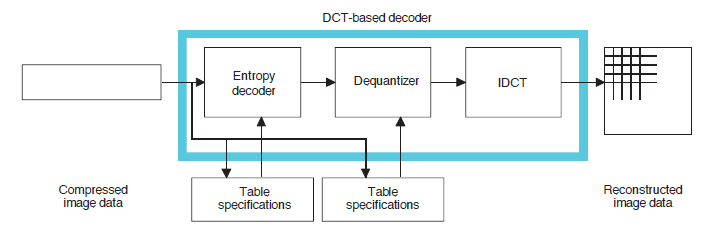
\includegraphics[width=\textwidth]{reverse}
\caption{Inverse JPEG de-compression (decoding).}
\end{figure}

\subsection{Forward and Inverse DCT}
An image is divided into non-overlapping blocks of size 8 x 8 and scanned left to right and top to bottom. Each block is transformed using a 2-dimensional DCT, which is given by:

\begin{equation}
F_{u,v} = \frac{1}{4}C_u C_v \sum_{x=0}^{7} \sum_{y=0}^{7}
	f(x,y)cos\frac{(2x+1)u\pi}{16}cos\frac{(2y+1)v\pi}{16}, \quad u,v = 0,\ldots ,7
\end{equation}

where $C_v$ follows the same rule as $C_u$ and

\begin{align*}
C_u = 
	\begin{dcases}
		1 \quad &\text{if $u\neq 0$,} \\
		\frac{1}{\sqrt{2}} &\text{if $u = 0$.}
	\end{dcases}
\end{align*}

The coefficients $F_{u,v}$ are coarsely approximated over a small set of possible values (quantization) and replaced by $\tilde{F}_{u,v}$. The quantization process introduces distortion and contributes to image quality loss.

With $\tilde{F}_{u,v}$ as the input (decoding), the inverse DCT can be applied to reconstruct an estimate of the block by:

\begin{equation}
\tilde{f}(x,y) = \frac{1}{4}  \sum_{u=0}^{7} \sum_{v=0}^{7} C_u C_v
\tilde{F}_{u,v} cos\frac{(2x+1)u\pi}{16} cos\frac{(2y+1)v\pi}{16}, \quad x,y=0,\ldots ,7
\end{equation}

where $C_v$ follows the same rule as $C_u$ and

\begin{align*}
C_u = 
	\begin{dcases}
		1 \quad &\text{if $u\neq 0$,} \\
		\frac{1}{\sqrt{2}} &\text{if $u = 0$.}
	\end{dcases}
\end{align*}

Once the DCT coefficients are calculated (in the forward encoding direction), the block is ordered in a zigzag pattern to improve spatial correlation and avoid edge cases. Figure \ref{zz:pattern} shows what this looks like.

\begin{figure}[ht]
\centering
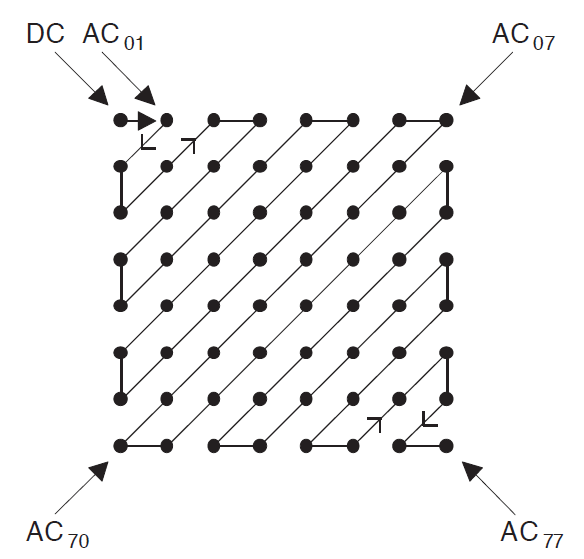
\includegraphics[width=0.4\textwidth]{zz}
\caption{Zig-Zag pattern}
\label{zz:pattern}
\end{figure}

\subsection{Quantization and Inverse Quantization}
The DCT works to find a 'best fit' axis. One way to think about it is a rotation of the $\mathbb{R}^{64}$ space aligning the coordinate system along the directions with largest variance. This only helps if we also simplify the representation of floating point numbers used to describe the DCT coefficients. This is what quantization does.

Quantization is the process of representing a variety of real numbers (for example measurements of an analog signal) using a preferably small set of integers.

The quantization step allows us to control the compression performance by reducing the set of possible values used to represent information. This step is where unrecoverable distortion is introduced by the JPEG algorithm.

\subsubsection*{Forward quantization}
Quantization in the JPEG standard (for all coefficients \textit{other} than the DC coefficient) is defined by:

\begin{equation}
F^q_{u,v} = floor \left( \frac{F_{u,v}}{loss-factor \times Q_{u,v}} + 0.5 \right).
\end{equation}

$Q_{u,v}$ is the entry $(u,v)$ of the standard quantization table listed in figure \ref{fig:Q} and \textit{loss-factor} is a user supplied parameter measuring the image quality to be lost during compression. Higher values of loss factor produce an image of lower quality.

\begin{figure}[ht]
\centering
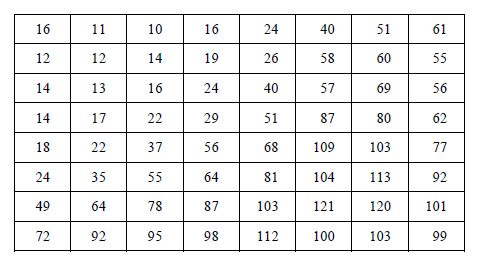
\includegraphics[width=0.6\textwidth]{Q}
\caption{JPEG standard quantization table $Q$.}
\label{fig:Q}
\end{figure}

\subsubsection{Inverse quantization}
The inverse quantization is defined by:

\begin{equation}
\tilde{F}_{u,v} = F^q_{u,v} \times loss-factor \times Q_{u,v}.
\end{equation}

An important quality of the quantization step is a number of coefficients which are rounded to zero during the forward quantization step. This is related to frequency, where high frequencies are lost before low frequencies. Thus, high frequency coefficients can be encoded with fewer bits.

After quantization and inverse quantization it is useful to calculate the Peak Signal to Noise Ratio (PNSR) defined as:

\begin{equation}
PSNR = 10log_{10} \left( \frac{255^2}{\frac{1}{N^2} \sum_{i,j=0}^{N-1} |f(i,j) - \tilde{f}(i,j)|^2} \right)
\end{equation}

\clearpage

\begin{figure}[ht]
	\centering
	\begin{subfigure}[h]{0.4\textwidth}
		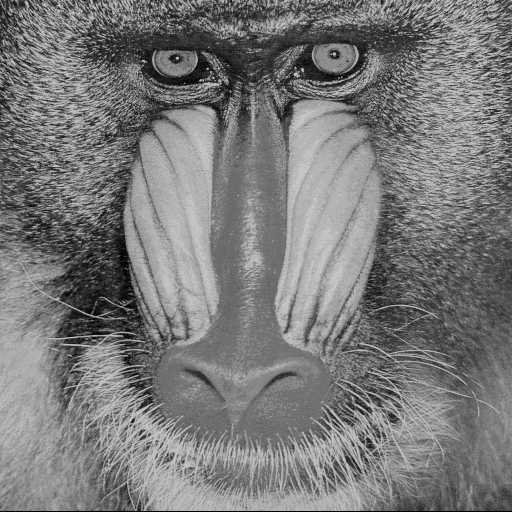
\includegraphics[width=\textwidth]{mandril_lf1}
		\caption{$loss-factor = 1$. $PSNR = 27.89dB$}
		\label{mandril:1}
	\end{subfigure}
	\par\bigskip
	\begin{subfigure}[h]{0.4\textwidth}
		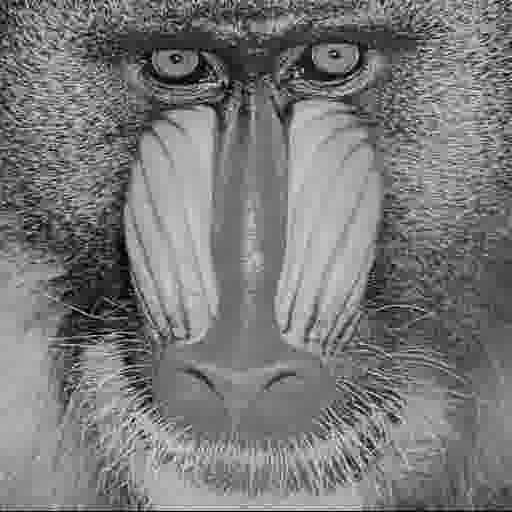
\includegraphics[width=\textwidth]{mandril_lf10}
		\caption{$loss-factor = 10$. $PSNR = 21.67dB$}
		\label{mandril:10}
	\end{subfigure}
	\par\bigskip
	\begin{subfigure}[h]{0.4\textwidth}
		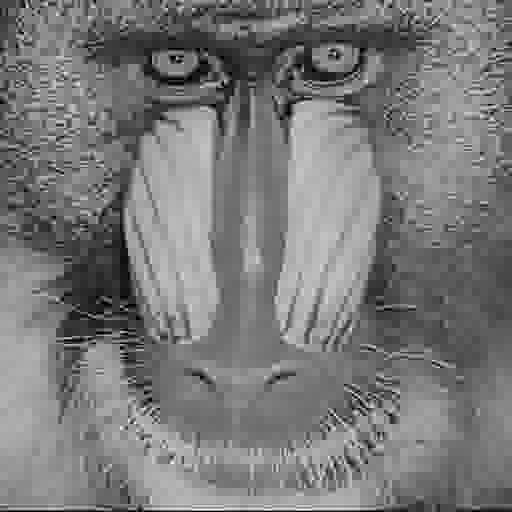
\includegraphics[width=\textwidth]{mandril_lf20}
		\caption{$loss-factor = 20$. $PSNR = 20.30dB$}
		\label{mandril:20}
	\end{subfigure}
	\caption{The results of varying \textit{loss-factor} for an image of a mandril.}
	\label{mandril:loss}
\end{figure}

\clearpage

\begin{figure}[ht]
	\centering
	\begin{subfigure}[h]{0.4\textwidth}
		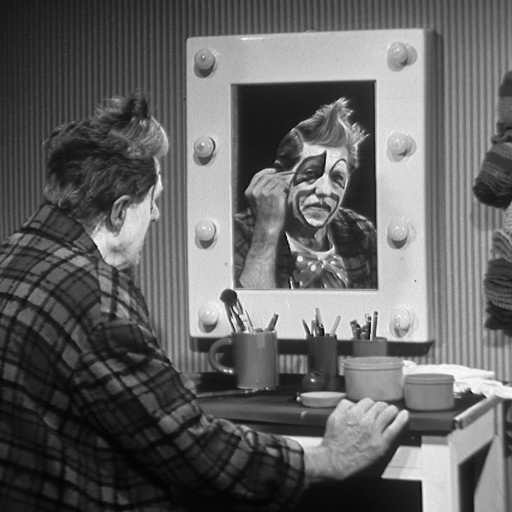
\includegraphics[width=\textwidth]{clown_lf1}
		\caption{$loss-factor = 1$. $PSNR = 36.40dB$}
		\label{clown:1}
	\end{subfigure}
	\par\bigskip
	\begin{subfigure}[h]{0.4\textwidth}
		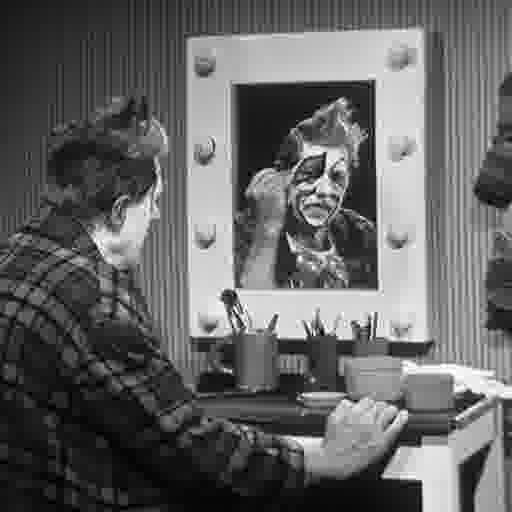
\includegraphics[width=\textwidth]{clown_lf10}
		\caption{$loss-factor = 10$. $PSNR = 27.65dB$}
		\label{clown:10}
	\end{subfigure}
	\par\bigskip
	\begin{subfigure}[h]{0.4\textwidth}
		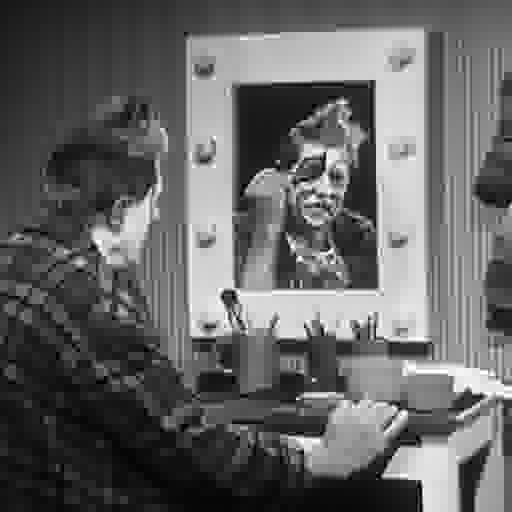
\includegraphics[width=\textwidth]{clown_lf20}
		\caption{$loss-factor = 20$. $PSNR = 25.08dB$}
		\label{clown:20}
	\end{subfigure}
	\caption{The results of varying \textit{loss-factor} for an image of a clown.}
	\label{clown:loss}
\end{figure}

\clearpage

\begin{figure}[ht]
	\centering
	\begin{subfigure}[h]{0.4\textwidth}
		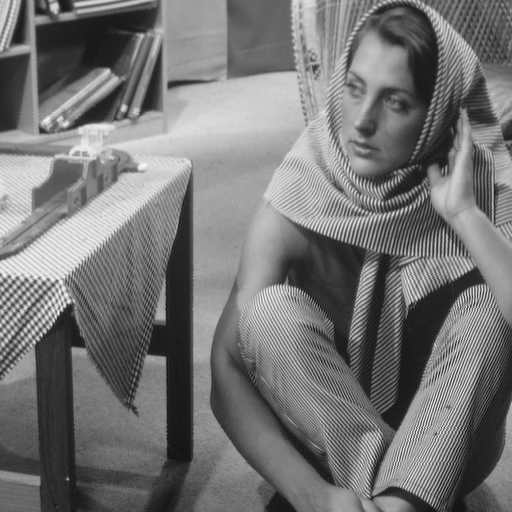
\includegraphics[width=\textwidth]{barbara_lf1}
		\caption{$loss-factor = 1$. $PSNR = 32.55dB$}
		\label{barbara:1}
	\end{subfigure}
	\par\bigskip
	\begin{subfigure}[h]{0.4\textwidth}
		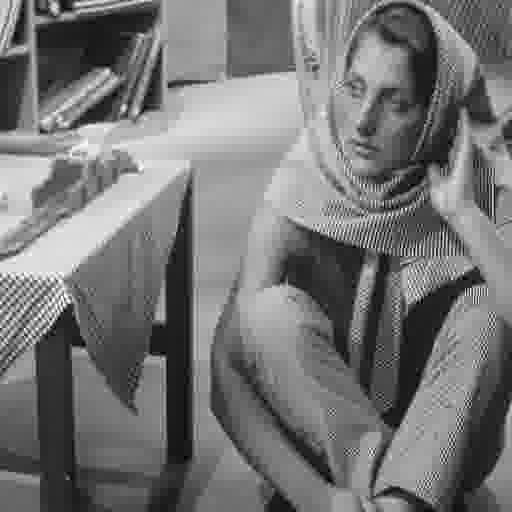
\includegraphics[width=\textwidth]{barbara_lf10}
		\caption{$loss-factor = 10$. $PSNR = 23.82dB$}
		\label{barbara:10}
	\end{subfigure}
	\par\bigskip
	\begin{subfigure}[h]{0.4\textwidth}
		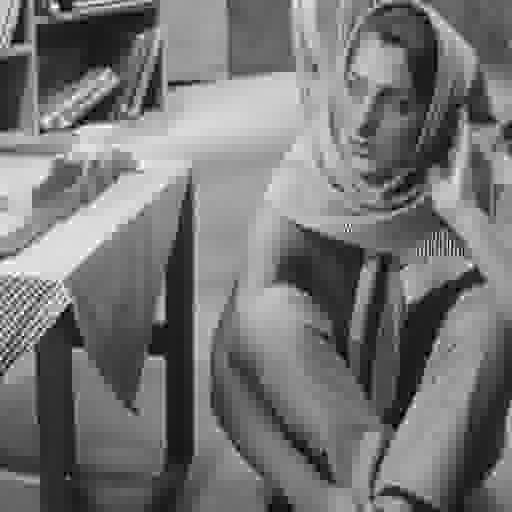
\includegraphics[width=\textwidth]{barbara_lf20}
		\caption{$loss-factor = 20$. $PSNR = 22.63dB$}
		\label{barbara:20}
	\end{subfigure}
	\caption{The results of varying \textit{loss-factor} for an image of a woman.}
	\label{barbara:loss}
\end{figure}
	
\clearpage

As you can see in figures \ref{mandril:loss}, \ref{clown:loss}, and \ref{barbara:loss}, higher values of \textit{loss-factor} lead to a lower quality image where details are lost to blocky squares and the PSNR decreases. It may be desirable to post-process these images with a low-pass filter or perform some sort of interpolation to smooth the processing artifacts, such as the "blockiness".

\subsection{Variable Length and Runlength Coding}
As hinted to previously, quantization produces some variable number of coefficients whose value is zero. Rather than encoding and storing/transmitting every coefficient, we can save some bits by counting sequences of zero values and encoding only the length of this "run-of-zeros". Of course this requires another level of data structuring in the compression scheme, both to encode and decode. The basic idea is to store only non-zero values and precede each value with a "codeword" indicating the number of preceding zeros to be inserted by the decoder.

Each block is encoded in this way and finally an End Of Block (EOB) symbol is encoded to signify the last significant symbol has been reach for that block. The decoder then fills the remainder of the block with zeros.

The idea is to package data as triplets:

\begin{align*}
\begin{bmatrix}
[nZeros & nBits & value]
\end{bmatrix}
\end{align*}

where 

\begin{itemize}
\item nZeros is the number of zeros preceding the value in the current entry.
\item nBits is the number of bits required to represent the coefficient value in two's complement. For the DC coefficient this is 12 bits and 11 bits for the AC coefficients.
\item value is the value of the coefficient
\end{itemize}

An EOB character simply sets $nZeros = 0$, $nBits = 0$, $value = 0$ and the next block is inserted immediately following.

This runlength encoding is then used as part of the encode/decode process before being used as input to an entropy coder.

\subsection{Entropy Coding}
Entropy coding aims to provide a lossless representation of a set of symbols whose average length is minimal. A variable length coding mechanism can be implemented where the most frequent data is coded with the shortest descriptions and longer descriptions are used for less frequent data. 

The JPEG standard supports both Huffman and arithmetic coding. Arithmetic encoding is more efficient. We will not implement either method.

\section{Conclusion}
This lab was difficult in concept. There are many steps to encoding and decoding the JPEG algorithm. Although the amount of code and the complexity of each small part was not large, keeping track of the data and organizing it in an efficient manner was the hard part. I did not have time to implement Entropy coding and learned some lessons about time-management in this lab. Overall, I don't think I'll ever be using my implementation of JPEG encoding/decoding when I know there are more robust, easier to use libraries already available, however I thought it was cool to get the chance to implement a real compression scheme.

\section{Appendix: Code}
\subsection{Helper Functions}
\begin{lstlisting}[language=python]
import numpy as np
import math
import scipy.fftpack
from PIL import Image

zz = np.asarray([
[0, 0],
[0, 1],
[1, 0],
[2, 0],
[1, 1],
[0, 2],
[0, 3],
[1, 2],
[2, 1],
[3, 0],
[4, 0],
[3, 1],
[2, 2],
[1, 3],
[0, 4],
[0, 5],
[1, 4],
[2, 3],
[3, 2],
[4, 1],
[5, 0],
[6, 0],
[5, 1],
[4, 2],
[3, 3],
[2, 4],
[1, 5],
[0, 6],
[0, 7],
[1, 6],
[2, 5],
[3, 4],
[4, 3],
[5, 2],
[6, 1],
[7, 0],
[7, 1],
[6, 2],
[5, 3],
[4, 4],
[3, 5],
[2, 6],
[1, 7],
[2, 7],
[3, 6],
[4, 5],
[5, 4],
[6, 3],
[7, 2],
[7, 3],
[6, 4],
[5, 5],
[4, 6],
[3, 7],
[4, 7],
[5, 6],
[6, 5],
[7, 4],
[7, 5],
[6, 6],
[5, 7],
[6, 7],
[7, 6],
[7, 7] ], np.int)

Q = np.asarray([
        [16, 11, 10, 16, 24, 40, 51, 61],
        [12, 12, 14, 19, 26, 58, 60, 55],
        [14, 13, 16, 24, 40, 57, 69, 56],
        [14, 17, 22, 29, 51, 87, 80, 62],
        [18, 22, 37, 56, 68, 109, 103, 77],
        [24, 35, 55, 64, 81, 104, 113, 92],
        [49, 64, 78, 87, 103, 121, 120, 101],
        [72, 92, 95, 98, 112, 100, 103, 99] ], np.float)

def dct_2D(A):
    #print(f'before = \n{A}\n')
    X = scipy.fftpack.dct(A, axis = 0, norm='ortho')
    Y = scipy.fftpack.dct(X, axis = 1, norm='ortho')
    #print(f'dct = \n{Y}\n')
    return Y

def idct_2D(A):
    Y = scipy.fftpack.idct(A, axis = 0, norm='ortho')
    X = scipy.fftpack.idct(Y, axis = 1, norm='ortho')
    #print(f'after = \n{X}\n')
    return X

def zigzag(A):
    #print(f'before zigzag = \n{A}\n\n')
    Y = np.zeros(64)
    for n in range(len(zz)):
        map = zz[n]
        Y[n] = A[map[0], map[1]]
    #print(f'after zigzag = \n{Y}\n\n')
    return Y

def izigzag(A):
    #print(f'before inverse zigzag = \n{A}\n\n')
    X = np.zeros((8, 8))
    for n in range(len(A)):
        map = zz[n]
        X[map[0], map[1]] = A[n]
    #print(f'after inverse zigzag = \n{X}\n\n')
    return X

def dctmgr(image, loss_factor):
    processed_image = np.zeros_like(image)
    dct_array = np.zeros((64, int(np.shape(image)[0] * np.shape(image)[1] / 64)))
    Ny, Nx = np.shape(image)
    nBlocksX = int(Nx/8)
    nBlocksY = int(Ny/8)
    block = 0
    # loop over 8x8 block cols
    for row in range(nBlocksX):
        for col in range(nBlocksY):
            indexX = col * 8
            indexY = row * 8
            # slice out an 8x8 block
            pix = image[indexY : indexY + 8, indexX : indexX + 8]
            #print(f'input = \n{pix}\n')
            # take 2D DCT transform
            dct_pix = dct_2D(pix)
            #print(f'dct = \n{dct_pix}\n')
            # quantize
            q = quant_coeffs(dct_pix, loss_factor)
            #print(f'q = \n{q}\n')
            # re-order block in zigzag pattern and place in output array
            zz = zigzag(q)
            #print(f'zz = \n{zz}\n')
            dct_array[:, block] = zz
            block += 1
    output = enc_rbv(dct_array)
    return output

def idctmgr(input, loss_factor):
    # decode rbv
    input = dec_rbv(input)
    nPix = int(np.shape(input)[1] / 8)
    output = np.zeros((nPix, nPix))
    # reconstruct image
    for col in range(np.shape(input)[1]):
        #print(f'input col = \n{input[:,col]}\n')
        indexX = (col % 64) * 8
        indexY = (int(col / 64)) * 8
        #print(f'index (row={indexX},col={indexY})\n')
        zag = izigzag(input[:, col])
        # invert quantization
        coeffs = iquant_coeffs(zag, loss_factor)
        #print(f'izz = \n{zag}\n')
        idct = idct_2D(coeffs)
        #print(f'idct = \n{idct}\n')
        output[indexY:indexY + 8, indexX:indexX + 8] = idct
    # clip values outside range(0,255)
    output = np.clip(output, 0, 255)
    return output

def quant_coeffs(A, loss_factor):
    #print(f'before quant = \n{A[0:8,0:8]}\n')
    #A[1:,:] = np.floor((np.divide(A[1:,:], zigzag(Q)[1:, np.newaxis]) / loss_factor) + 0.5)
    z = A[0,0]
    A = np.floor((A / (loss_factor * Q)) + 0.5)
    A[0,0] = z
    #print(f'after quant = \n{A[0:8,0:8]}\n')
    return A

def iquant_coeffs(A, loss_factor):
    #A[1:,:] = A[1:,:] * loss_factor * zigzag(Q)[1:, np.newaxis
    z = A[0,0]
    A = A * loss_factor * Q
    A[0,0] = z
    #print(f'after iquant = \n{A[0:8,0:8]}\n')
    return A

def enc_rbv(A):
    symb = np.zeros((0,3), np.int16)
    for i in range(np.shape(A)[1]):
        # Handle DC coeff
        symb = np.vstack([symb, [0, 12, A[0,i]]])

        # Handle AC coeffs. nzi means non-zero indices
        tmp = A[:,i].flatten()
        nzi = np.where(tmp[1:] != 0)[0]
        prev_index = 0
        for k in range(len(nzi)):
            curr_index = nzi[k] + 1
            zeros = curr_index - prev_index - 1
            prev_index = curr_index
            symb = np.vstack([symb, [zeros, 11, tmp[curr_index]]])
        symb = np.vstack([symb, [0,0,0]])
        #print(f'symb = \n{symb}\n')
    return symb

def dec_rbv(symb):
    output = np.zeros((64, 4096), np.int16)
    EOB = np.asarray([0, 0, 0], np.int16)
    symb_row = 0
    row = 0
    col = 0
    zeros = 0
    # loop over symb matrix to reconstruct blocks separated by EOB vectors
    while symb_row < np.shape(symb)[0]:
        if np.array_equal(symb[symb_row], EOB):
            # EOB
            row = 0
            col += 1
            symb_row += 1
        else:
            # reconstruct row of coefficient matrix
            row += int(symb[symb_row, 0])
            output[row, col] = symb[symb_row, 2]
            row += 1
            symb_row += 1
    return output
    
\end{lstlisting}

\subsection{Main}
    \begin{lstlisting}[language=python]
from tkinter import filedialog
import matplotlib.pyplot as plt
import numpy as np
from PIL import Image
import lab_functions as lf

# UI dialog to select files -> selection of multiple files will run all functions for each file
files = filedialog.askopenfilenames()
for f in files:
    filename = str.split(f,'/')[-1]
    filename = str.split(filename,'.')[0]
    filepath = f

    image = np.asarray(Image.open(f))
    Image.fromarray(image).save('figures/' + filename + '.png')

    loss_factor = 1
    processed = lf.dctmgr(image, loss_factor)
    x = lf.idctmgr(processed, loss_factor)
    Image.fromarray(x.astype(np.uint8)).save('figures/' + filename + '_lf' + str(loss_factor) + '.png')

    loss_factor = 10
    processed = lf.dctmgr(image, loss_factor)
    x = lf.idctmgr(processed, loss_factor)
    Image.fromarray(x.astype(np.uint8)).save('figures/' + filename + '_lf' + str(loss_factor) + '.png')
    
    loss_factor = 20
    processed = lf.dctmgr(image, loss_factor)
    x = lf.idctmgr(processed, loss_factor)
    Image.fromarray(x.astype(np.uint8)).save('figures/' + filename + '_lf' + str(loss_factor) + '.png')

print('done')
\end{lstlisting}

\end{document}